\documentclass{article}\usepackage[]{graphicx}\usepackage[]{xcolor}
% maxwidth is the original width if it is less than linewidth
% otherwise use linewidth (to make sure the graphics do not exceed the margin)
\makeatletter
\def\maxwidth{ %
  \ifdim\Gin@nat@width>\linewidth
    \linewidth
  \else
    \Gin@nat@width
  \fi
}
\makeatother

\definecolor{fgcolor}{rgb}{0.345, 0.345, 0.345}
\newcommand{\hlnum}[1]{\textcolor[rgb]{0.686,0.059,0.569}{#1}}%
\newcommand{\hlstr}[1]{\textcolor[rgb]{0.192,0.494,0.8}{#1}}%
\newcommand{\hlcom}[1]{\textcolor[rgb]{0.678,0.584,0.686}{\textit{#1}}}%
\newcommand{\hlopt}[1]{\textcolor[rgb]{0,0,0}{#1}}%
\newcommand{\hlstd}[1]{\textcolor[rgb]{0.345,0.345,0.345}{#1}}%
\newcommand{\hlkwa}[1]{\textcolor[rgb]{0.161,0.373,0.58}{\textbf{#1}}}%
\newcommand{\hlkwb}[1]{\textcolor[rgb]{0.69,0.353,0.396}{#1}}%
\newcommand{\hlkwc}[1]{\textcolor[rgb]{0.333,0.667,0.333}{#1}}%
\newcommand{\hlkwd}[1]{\textcolor[rgb]{0.737,0.353,0.396}{\textbf{#1}}}%
\let\hlipl\hlkwb

\usepackage{framed}
\makeatletter
\newenvironment{kframe}{%
 \def\at@end@of@kframe{}%
 \ifinner\ifhmode%
  \def\at@end@of@kframe{\end{minipage}}%
  \begin{minipage}{\columnwidth}%
 \fi\fi%
 \def\FrameCommand##1{\hskip\@totalleftmargin \hskip-\fboxsep
 \colorbox{shadecolor}{##1}\hskip-\fboxsep
     % There is no \\@totalrightmargin, so:
     \hskip-\linewidth \hskip-\@totalleftmargin \hskip\columnwidth}%
 \MakeFramed {\advance\hsize-\width
   \@totalleftmargin\z@ \linewidth\hsize
   \@setminipage}}%
 {\par\unskip\endMakeFramed%
 \at@end@of@kframe}
\makeatother

\definecolor{shadecolor}{rgb}{.97, .97, .97}
\definecolor{messagecolor}{rgb}{0, 0, 0}
\definecolor{warningcolor}{rgb}{1, 0, 1}
\definecolor{errorcolor}{rgb}{1, 0, 0}
\newenvironment{knitrout}{}{} % an empty environment to be redefined in TeX

\usepackage{alltt}
\usepackage[utf8]{inputenc}
\usepackage{amsfonts}
\usepackage{tgpagella}
\usepackage{graphicx} % Required for inserting images
\usepackage{polski}
\renewcommand*{\figurename}{Rysunek}
\usepackage{nicefrac, xfrac}
\usepackage[margin=1in]{geometry}
\usepackage{hyperref}
\usepackage{xcolor}
\usepackage{amssymb}
\usepackage[bottom]{footmisc}
\usepackage{float}

\date{\now}
\IfFileExists{upquote.sty}{\usepackage{upquote}}{}
\begin{document}

\begin{titlepage}
\end{titlepage}
\begin{center}
 {\LARGE\bfseries Projekt\\}
 \vspace{0.5cm}
 {\Huge\bfseries \color{magenta} Pimp My Wheels\\}
 \vspace{0.5cm}
 {\LARGE\bfseries Bazy danych\\}
 {\Large Prowadzący kurs: dr Tomasz Stroiński\\}
 % ----------------------------------------------------------------
 \vspace{1cm}
 {\Large\bfseries Autorzy:\\[4pt]}
 \vspace{1.5cm}
  {\Large\bfseries Weronika Kuzara\\[3pt]}
  \vspace{0.5cm}
 
 {\Large\bfseries Martyna Maciaszek\\[3pt]}
 \vspace{0.5cm}
 
 {\Large\bfseries Aleksander Rzyhak\\[3pt]}
 \vspace{0.5cm}
 
 {\Large\bfseries Oskar Matysik\\[3pt]}
 \vspace{0.5cm}
 
 {\Large\bfseries Aleksandra Palka\\[5pt]}
  % ----------------------------------------------------------------

 \vfill
{\Large \today}
\end{center}
\newpage



\section{Wstęp}
Raport jest przedostatnią częścią projektu polagającego na stworzeniu bazy danych warsztatu „Pimp My Wheels”. Został zaprojektowany schemat bazy danych, na podstawie którego została stworzona już właściwa baza. Następnie została ona wypełniona losowymi danymi.

Raport ma na celu przeanalizowanie działalności warsztatu „Pimp My Wheels” znajdującego się we Wrocławiu. Na moment, dla którego pisany był raport, warsztat działa od początku 2014 roku do końca 2017 roku. Firma zajmuje się prowadzeniem klasycznego warsztatu oraz skupem, renowacją i sprzedażą samochodów i motocykli. 

\section{Odsetek naprawianych marek pojazdów}
%Odsetek naprawianych marek pojazdów.

Przeprowadzono analizę, aby sprawdzić jakich marek pojazdy najczęściej pojawiają się w warsztacie do naprawy. 



Można przedstawić procentowy udział marek pojazdów klientów salonu, zaczynając od najczęściej się pojawiającej:

\begin{verbatim}
1. Volkswagen: 14.57%
2. Opel: 9.38%
3. Ford: 8.58%
4. Renault: 8.38%
5. Audi: 5.39%
6. SEAT: 4.59%
7. Skoda: 4.19%
8. Fiat: 4.19%
9. Mercedes-Benz: 3.79%
10. Hyundai: 3.59%
11. BMW: 3.39%
12. Toyota: 2.79%
13. Hero: 2.4%
14. Peugeot: 2.4%
15. smart: 2.4%
16. Bajaj: 2%
17. Kia: 1.6%
18. Honda: 1.6%
19. Dacia: 1.4%
20. Suzuki: 1.4%
21. Nissan: 1.2%
22. Citroen: 1.2%
23. Yamaha: 1.2%
24. Mazda: 1%
25. MINI: 0.8%
26. Royal: 0.8%
27. Porsche: 0.8%
28. Volvo: 0.6%
29. Jaguar: 0.6%
30. KTM: 0.6%
31. Lexus: 0.4%
32. Land: 0.4%
33. Jeep: 0.4%
34. Cupra: 0.4%
35. Harley-Davidson: 0.2%
36. Chevrolet: 0.2%
37. Mitsubishi: 0.2%
38. Subaru: 0.2%
39. Alpina: 0.2%
40. TVS: 0.2%
41. Kawasaki: 0.2%
42. Aprilia: 0.2%
\end{verbatim}

Jak widać, najpopularniejsze są pojazdy marki Volkswagen. Pojazdy tej marki stanowią 14.57\% wszystkich. \\

Najmniej popularne są marki Chevrolet, Mitsubishi, Subaru, Alpina, TVS, Kawasaki, Aprilia i Harley-Davidson. Każdą z nich reprezentowało 0.20\% pojazdów, które się pojawiły w warsztacie. Ilość pojazdów, które były w warsztacie to 501. Było więcej samochodów niż motorów. Różnica między ilością obu typów pojazdu wynosiła 399, a samochodów było 450.

Sprawdzono także, jak prezentowałyby się rozkład marek, gdyby brano pod uwagę jedynie samochody



Można przedstawić ranking marek, zaczynając od najczęściej się pojawiającej:

\begin{verbatim}
1. Volkswagen: 16.22%
2. Opel: 10.44%
3. Ford: 9.56%
4. Renault: 9.33%
5. Audi: 6%
6. SEAT: 5.11%
7. Fiat: 4.67%
8. Skoda: 4.67%
9. Mercedes-Benz: 4.22%
10. Hyundai: 4%
11. BMW: 3.78%
12. Toyota: 3.11%
13. smart: 2.67%
14. Peugeot: 2.67%
15. Kia: 1.78%
16. Dacia: 1.56%
17. Citroen: 1.33%
18. Nissan: 1.33%
19. Mazda: 1.11%
20. Porsche: 0.89%
21. MINI: 0.89%
22. Volvo: 0.67%
23. Jaguar: 0.67%
24. Suzuki: 0.67%
25. Jeep: 0.44%
26. Lexus: 0.44%
27. Land: 0.44%
28. Cupra: 0.44%
29. Mitsubishi: 0.22%
30. Chevrolet: 0.22%
31. Alpina: 0.22%
32. Subaru: 0.22%
\end{verbatim}

Wśród aut prym wiedzie Volkswagen, reprezentując  16.22\% naprawianych samochodów. Najmniej było samochodów marek Chevrolet, Alpina, Subaru i Mitsubishi. Było ich 0.22\% dla każdej. \\

Pozostały do sprawdzenia motory.



Udział procentowy poszczególnych marek wśród nich prezentuje się następująco:

\begin{verbatim}
1. Hero: 23.53%
2. Bajaj: 19.61%
3. Honda: 15.69%
4. Yamaha: 11.76%
5. Royal: 7.84%
6. Suzuki: 7.84%
7. KTM: 5.88%
8. Aprilia: 1.96%
9. TVS: 1.96%
10. Kawasaki: 1.96%
11. Harley-Davidson: 1.96%
\end{verbatim}

Wśród nich najczęściej naprawiano motory marki Hero. Pojazdy tej marki stanowią 23.53\% wszystkich. Najmniej popularnymi motorami są z kolei modele marek TVS, Kawasaki, Harley-Davidson i Aprilia. W warsztacie było zaledwie 1.96\% motorów każdej z wymienionych marek.

\section{Liczba naprawianych pojazdów w każdym miesiącu pracy warsztatu}

\begin{knitrout}
\definecolor{shadecolor}{rgb}{0.969, 0.969, 0.969}\color{fgcolor}\begin{figure}[H]

{\centering 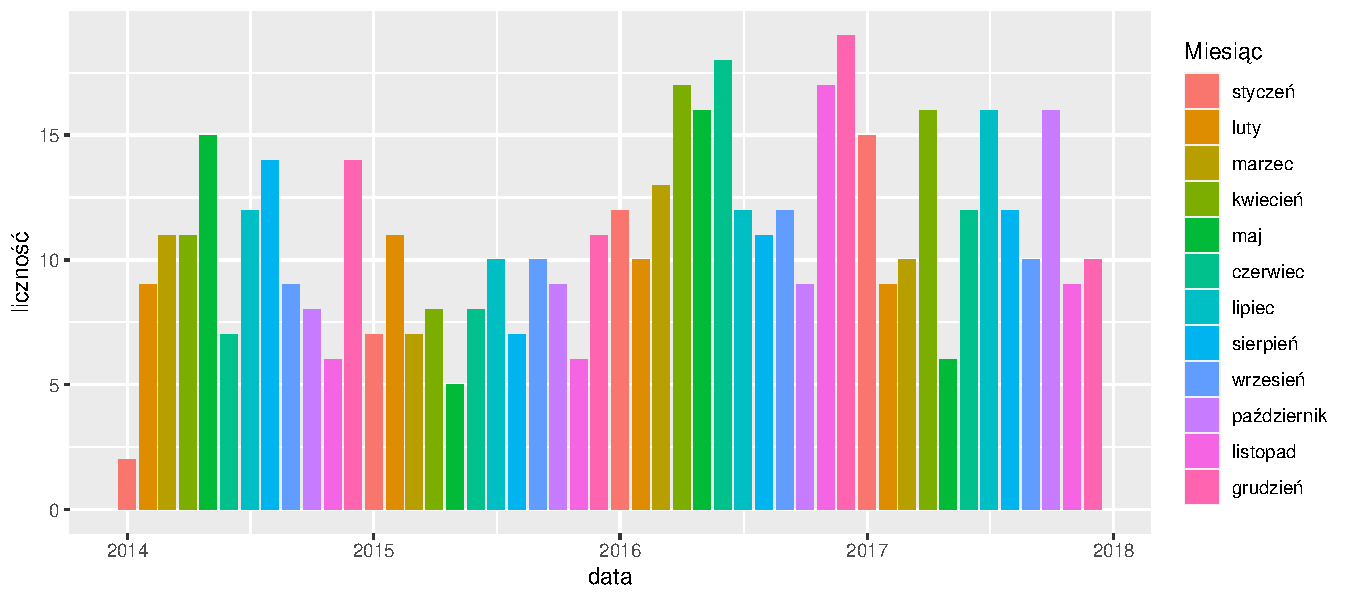
\includegraphics[width=\maxwidth]{figure/fig_naprawy_miesiecznie-1} 

}

\caption[Wykres liczba naprawianych pojazdów w każdym miesiącu pracy warsztatu]{Wykres liczba naprawianych pojazdów w każdym miesiącu pracy warsztatu}\label{fig:fig_naprawy_miesiecznie}
\end{figure}

\end{knitrout}

Wykres \ref{fig:fig_naprawy_miesiecznie} przedstawia liczbę naprawionych pojazdów w każdym miesiącu pracy warsztatu. Najwięcej pojazdów zostało naprawionych w miesiącach 
grudzień 2014, maj 2017,
a było ich 18. Natomiast najmniej przeprowadzonych napraw było w miesiącu
styczeń 2014,
było ich 0. Średnia liczba napraw miesięcznie wynosi 
10.44. 

\section{Tabela najlepszych okazji}

Zostanie teraz omówiona tabela najlepszych okazji, czyli pojazdów skupionych i sprzedanych, które przyniosły najwięcej zysku. Został uwzględniony także koszt naprawy pojazdu, gdy była ona potrzebna.





\begin{knitrout}
\definecolor{shadecolor}{rgb}{0.969, 0.969, 0.969}\color{fgcolor}\begin{kframe}
\begin{verbatim}
##     id_samochodu         marka    model   zysk
## 58            65          Audi       S5 143474
## 679          927 Mercedes-Benz C 63 AMG 130010
## 452          609           BMW       X3 118888
## 309          432         Tesla  Model S 114604
## 507           65          Audi       S5 103300
\end{verbatim}
\end{kframe}
\end{knitrout}

Największy zysk ze sprzedaży pojazdu warsztat odniósł dla pojazdu o id 65. Jest nim Audi o modelu S5. Warsztat zarobił on na nim około 143.47 tys. zł. 
Na drugim miejscu znajduje się Mercedes-Benz o modelu C 63 AMG. Zysk z tego pojazdu wyniósł około 130.01 tys. zł, czyli o około 13.46 tys. zł mniej niż dla pojazdu znajdującego się na pierwszym miejscu, czyli różnica w cenie jest duża.
W trzeciej kolejności najwięcej zarobił pojazd BMW o modelu X3, na którym warsztat zarobił około 118.89 tys. zł. Jest to mniej od poprzedniego pojazdu o około 11.12 tys. zł, czyli różnica w cenie jest duża. 
Ogólnie każdy pojazd znajdujący się w top 5 najlepszych okazji przyniósł zysk wielkości przynajmnej 100 tyś. zł.

\section{Profil klienta}

W następnej kolejności zostaną przeanalizawani klienci warsztatu. Zostaną sprawdzone liczności klientów ze względu na różne ich cechy.

\subsection{Płeć}

Pierwszą cechą wziętą pod uwagę jest płeć klienta. Zostanie sprawdzone, ile jest kobiet i mężczyzn wśród naszych klientów oraz jak duża jest różnica w licznościach tych grup.

\begin{knitrout}
\definecolor{shadecolor}{rgb}{0.969, 0.969, 0.969}\color{fgcolor}\begin{figure}[H]

{\centering 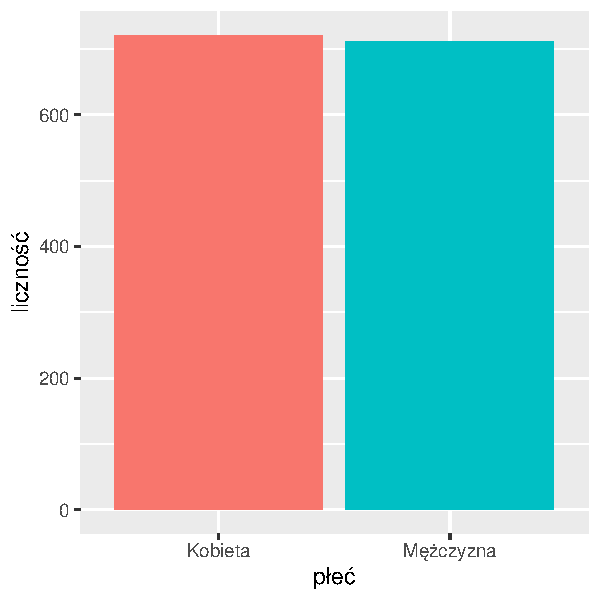
\includegraphics[width=\maxwidth]{figure/fig_plec-1} 

}

\caption[Wykres liczby klientów przy podziale ze względu na płeć]{Wykres liczby klientów przy podziale ze względu na płeć}\label{fig:fig_plec}
\end{figure}

\end{knitrout}

Na wykresie słupkowym \ref{fig:fig_plec} są zaprezentowane liczności klientów przy podziale ze względu na płeć. Więcej klientów warsztatu należy do grupy mężczyzn, jest ich 749. Grupa mężczyzn jest około 1.055
razy większa od grupy kobiet (jest ich 710), a zatem różnica jest nieduża.

\subsection{Wiek}

Zostanie również przeanalizowany rozkład wieku klientów warsztatu.





\begin{knitrout}
\definecolor{shadecolor}{rgb}{0.969, 0.969, 0.969}\color{fgcolor}\begin{figure}[H]

{\centering 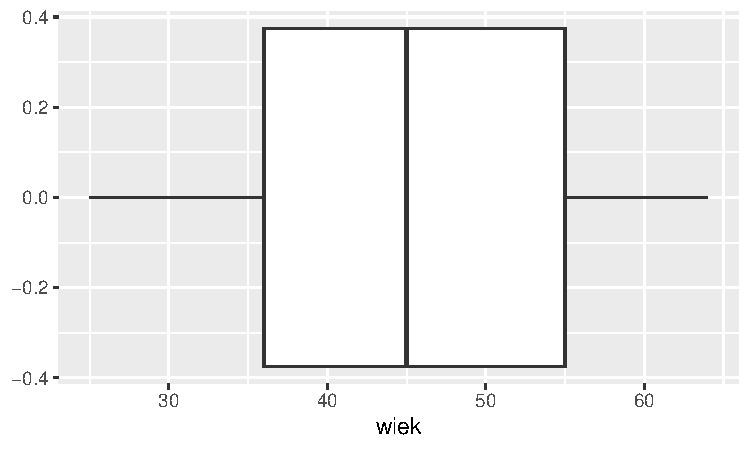
\includegraphics[width=\maxwidth]{figure/fig_wiek-1} 

}

\caption[Wykres pudełkowy wieku klientów]{Wykres pudełkowy wieku klientów}\label{fig:fig_wiek}
\end{figure}

\end{knitrout}

Rysunek \ref{fig:fig_wiek} przedstawia wykres pudełkowy wieku klientów warsztatu. Widać, że mediana wieku wynosi 46 lat, natomiast pierwszy kwartyl wynosi 37 lat, a trzeci kwartyl 56 lat. Zatem połowa klientów warsztatu jest wieku między 37 lat a 56 lat.
Najmłodszy klient warsztatu ma 25 lat, natomiast najstarszy jest w wieku 64 lat.



\begin{table}[H]
\centering
\begin{tabular}{c|c} \hline
Miara & Wartość \\ \hline
Średnia & 45.86 \\ 
Odchylenie standardowe & 10.99 \\
Skośność & -0.06  \\ 
Kurtoza & 1.79 \\ \hline
\end{tabular}
\caption{Wybrane miary wieku klientów}
\label{tab_wiek}
\end{table}

Kilka miar, których nie da się odczytać z wykresu pudełkowego, zostało przedstawionych w tabeli \ref{tab_wiek}. Można zatem odczytać, że średnio klieci mają 45.86 lat, a odchylenie standardowe wieku wynosi 10.99 lat. Wartość współczynnika skośności jest bliska 0, a zatem rozkład wieku można uznać za symetryczny. Kurtoza przyjmuje wartość większą od 0, a zatem rozkład wieku jest leptokurtyczny, czyli jest bardziej wysmukły niż normalny.

\subsection{Miasto}
\begin{knitrout}
\definecolor{shadecolor}{rgb}{0.969, 0.969, 0.969}\color{fgcolor}\begin{kframe}
\begin{verbatim}
##   miejsce              miasto liczność
## 1     1.0             Wrocław      743
## 2     2.0        Zielona Góra       23
## 3     3.5 Gorzów Wielkopolski       20
## 4     3.5            Warszawa       20
## 5     5.0              Poznań       18
\end{verbatim}
\end{kframe}
\end{knitrout}

Najwięcej klientów warsztatu pochodzi z miasta Wrocław. Liczniść w nim wynosi 743 klientów. W następnej kolejności najwięcej klientów pochodzi z miasta Zielona Góra, z czego liczność w nim wynosi 23 klientów, czyli jest ich 32.3 mniej niż klientów z miasta Wrocław. Na miejscu 3.5 są miasta Gorzów Wielkopolski, Warszawa, mieszka w nich 20 klientów. Natomiast na ostatnim miejscu przedstawionym w tabeli jest miasto Poznań, mieszka w nim 18 klientów.

\subsection{Karta lojalnościowa}

W tej części zostanie sprawdzone ilu klientów posiada kartę lojalnościową. Klient zdobywa ją po skorzystaniu z usług warsztatu (naprawa, zakup lub sprzedaż pojazdu) przynajmniej trzy razy. Klient posiadający tę kartę może kupować samochody ze zniżką w wysokości 3\%.

\begin{knitrout}
\definecolor{shadecolor}{rgb}{0.969, 0.969, 0.969}\color{fgcolor}\begin{figure}[H]

{\centering 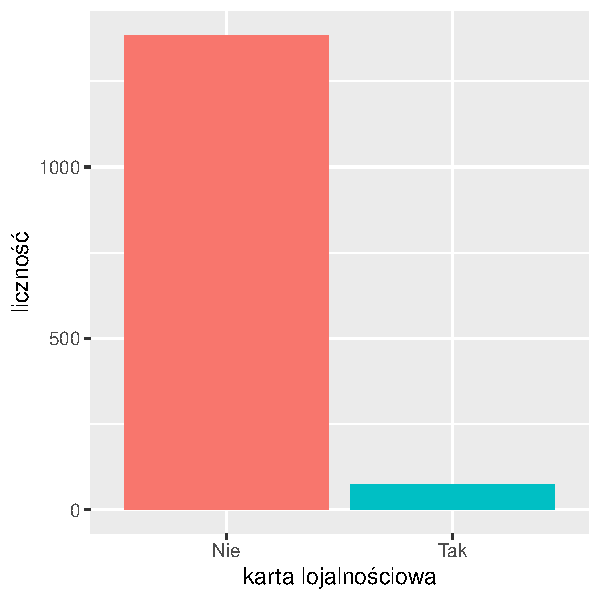
\includegraphics[width=\maxwidth]{figure/fig_karta-1} 

}

\caption[Wykres liczby klientów ze względu na posiadanie karty lojalnościowej]{Wykres liczby klientów ze względu na posiadanie karty lojalnościowej}\label{fig:fig_karta}
\end{figure}

\end{knitrout}

Bardziej liczną grupą są klienci, którzy nie posiadają karty lojalnościowej, jest ich 1385 (95\% wszystkich klientów). W grupie klientów, którzy posiadają kartę lojalnościową, jest 74 osób i stanowią oni 5\% klientów warsztatu.

\section{Jak wybrane cechy pojazdów wpływają na zysk warsztatu?}

W tym paragrafie zostaną opisane zależności między zyskiem ze sprzedaży pojazdów, skupionych i w razie potrzeby naprawionych przez warsztat, a cechami: rodzaj pojazdu, czy jest powypadkowy i pojemność silnika.

\subsection{Rodzaj pojazdu}

Pierwszą cechą braną pod uwagę jest rodzaj pojazdu, czyli czy jest to samochód czy motocykl.

\begin{knitrout}
\definecolor{shadecolor}{rgb}{0.969, 0.969, 0.969}\color{fgcolor}\begin{figure}[H]

{\centering 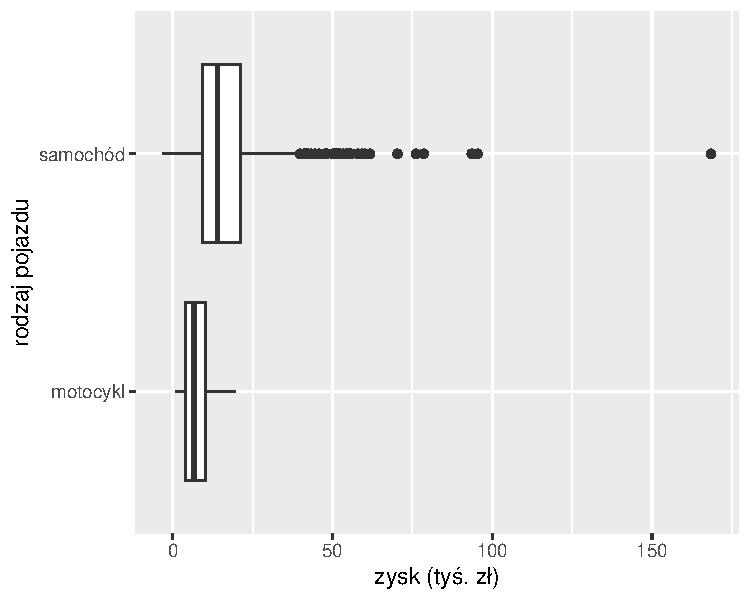
\includegraphics[width=\maxwidth]{figure/fig_typ-1} 

}

\caption[Wykresy pudełkowe zysku ze względu na rodzaj pojazdu]{Wykresy pudełkowe zysku ze względu na rodzaj pojazdu}\label{fig:fig_typ}
\end{figure}

\end{knitrout}

Na rysunku \ref{fig:fig_typ} przedstawione są dwa wykresy pudełkowe zysków, jeden dla samochodów, drugi dla motocykli. Większa mediana, wynosząca 14.22, jest dla pojazdów typu samochód. W drugiej grupie wynosi ona 8.85 tyś. zł. 
Większy pierwszy kwartyl występuje w grupie typu samochód, wynosi on 9.63 tyś. zł, w porównaniu dla grupy typu motocykl jego wartość wynosi 5.15 tyś. zł.
W przypadku kwartyla trzeciego większa wartość występuje w grupie typu samochód (wynosi 22.18 tyś. zł). W drugiej grupie wynosi on 13.01 tyś. zł.
Największy zysk przyniósł samochód, a wyniósł on 143 tyś. zł. 
Najmniejszy zysk natomiast przyniósł samochód i wyniósł on -3 tyś. zł. Zatem częściej większy zysk dla warsztatu przynosi sprzedaż pojazdów typu samochód. 

\subsection{Czy powypadkowy}

Następną badaną cechą jest to, czy pojazd jest powypadkowy.

\begin{knitrout}
\definecolor{shadecolor}{rgb}{0.969, 0.969, 0.969}\color{fgcolor}\begin{figure}[H]

{\centering 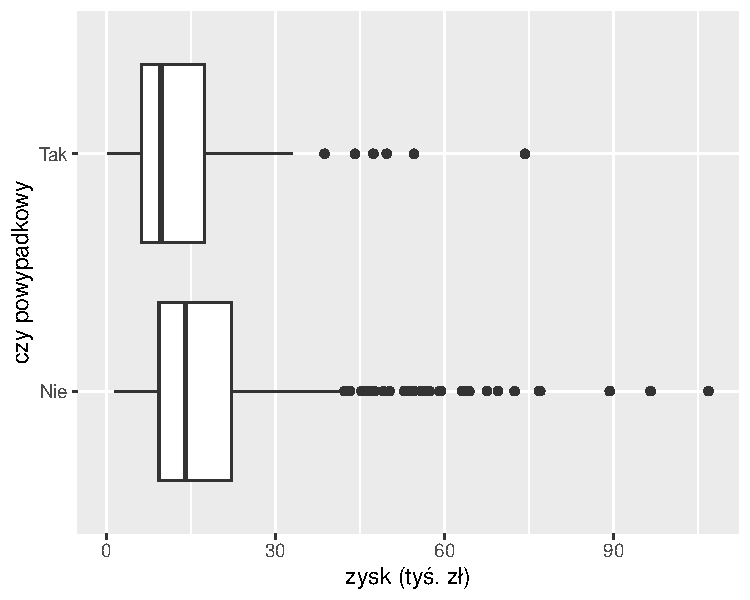
\includegraphics[width=\maxwidth]{figure/fig_wypadkowy-1} 

}

\caption[Wykresy pudełkowe zysku ze względu na to czy pojazd jest powypadkowy]{Wykresy pudełkowe zysku ze względu na to czy pojazd jest powypadkowy}\label{fig:fig_wypadkowy}
\end{figure}

\end{knitrout}

Na rysunku \ref{fig:fig_wypadkowy} przedstawione są dwa wykresy pudełkowe zysków dla pojazdów powypadkowych i niepowypadkowych. Większa mediana, wynosząca 14.22 tyś. zł, jest dla pojazdów niepowypadkowych. W drugiej grupie wynosi ona 11.56 tyś. zł. 
Większy pierwszy kwartyl występuje w grupie pojazdów niepowypadkowych, wynosi on 9.69 tyś. zł, w porównaniu dla grupy pojazdów powypadkowych jego wartość wynosi 8 tyś. zł.
Większa wartość trzeciego kwartylu występuje dla pojazdów niepowypadkowych i wynosi 22.87 tyś. zł. Dla pojazdów powypadkowych wynosi on 17.04 tyś. zł.
Największy zysk przyniósł pojazd z grupy niepowypadkowych i wyniósł on 143.47 tyś. zł. 
Najmniejszy zysk natomiast przyniósł pojazd z grupy niepowypadkowych i wyniósł on -3.2 tyś. zł. Zatem częściej większy zysk dla warsztatu przynosi sprzedaż pojazdów niepowypadkowych. 

\subsection{Pojemność silnika}

Ostatnią cechą braną pod uwagę jest pojemność silnika pojazdu.

\begin{knitrout}
\definecolor{shadecolor}{rgb}{0.969, 0.969, 0.969}\color{fgcolor}\begin{figure}[H]

{\centering 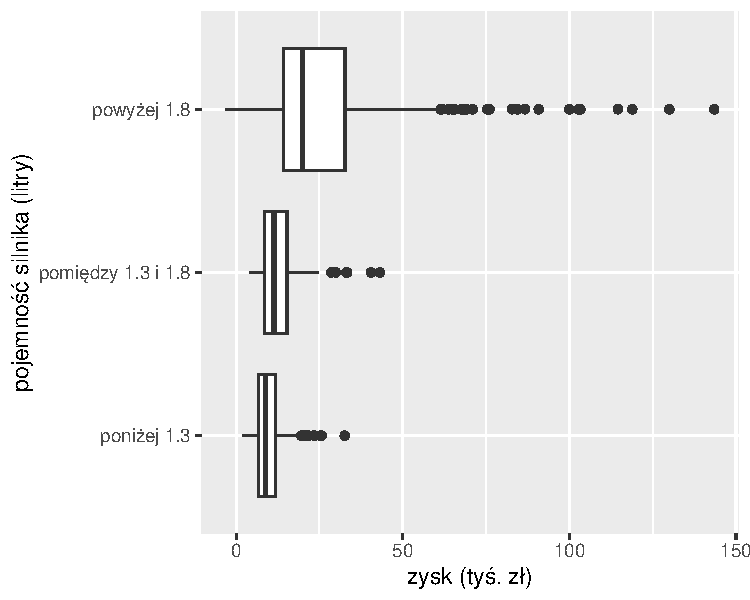
\includegraphics[width=\maxwidth]{figure/fig_pojemnosc-1} 

}

\caption[Wykresy pudełkowe zysku ze względu na pojemność silnika]{Wykresy pudełkowe zysku ze względu na pojemność silnika}\label{fig:fig_pojemnosc}
\end{figure}

\end{knitrout}

Na rysunku \ref{fig:fig_wypadkowy} przedstawione są wykresy pudełkowe zysków ze względu na pojemność silnika. Największa mediana, wynosząca 19.9 tyś. zł, jest dla pojazdów o pojemności silnika powyżej 1.8 litra. Natomiast najmniej ona wynosi 8.86 tyś. zł w grupie pojazdów o pojemności poniżej 1.3 litra. 
Największy pierwszy kwartyl występuje w grupie pojazdów o pojemności powyżej 1.8 litra, wynosi on 14.22 tyś. zł, w porównaniu z pojazdami o pojemności poniżej 1.3 litra, dla których jego wartość jest najmniejsza i wynosi 6.6 tyś. zł.
Największa wartość trzeciego kwartylu występuje dla pojazdów o pojemności powyżej 1.8 litra i wynosi 32.7 tyś. zł. Dla pojazdów poniżej 1.3 litra wynosi on 11.77 tyś. zł i jest to najmnijesza wartość w tych grupach.
Największy zysk przyniósł pojazd o pojemności silnika powyżej 1.8 litra i wyniósł on 143.47 tyś. zł. 
Najmniejszy zysk natomiast przyniósł pojazd z pojemnością silnika powyżej 1.8 litra i wyniósł on -3.2 tyś. zł. Zatem przeważnie największy zysk dla warsztatu przynosi sprzedaż pojazdów o pojemności silnika powyżej 1.8 litra. Najczęściej najmniejszy zysk przynosi sprzedaż pojazdów z pojemnością silnika poniżej 1.3 litra.

\section{Kim są najlepszy mechanik i sprzedawca w warsztacie?}

Przez czas działania warsztatu „Pimp My Wheels” osoba zarządzająca warsztatem nie była skłonna do dawania podwyżek, jednak postanowiła zlecić informatykowi by przeanalizował bazę danych i znalazł pracowników, którzy zasługują na większe wynagrodzenie. \\

Warsztatowi zależy na tym by sprzedawca zarobił dla firmy dużą kwotę (Może to osiągnąć sprzedając bardzo dużo pojazdów albo sprzedając wartościowe pojazdy), ale także by był charyzmatyczny i był w stanie przekonać wiele osób do zakupu. Rozważone wobec tego zostanie to który obecnie pracujący sprzedawca przekonał klientów do kupna największej liczby pojazdów, a który odpowiada za najwięcej środków pochodzących ze sprzedaży. \\


Tabela, w której są dane o sprzedawcach  pracujących w dowolnym momencie w warsztacie wygląda następująco:

{\color{red}[tu wstaw tamto]} 

\begin{knitrout}
\definecolor{shadecolor}{rgb}{0.969, 0.969, 0.969}\color{fgcolor}\begin{kframe}
\begin{verbatim}
##              mechanik   suma ile_napraw płaca id_pracownika status
## 1        Lena Olejnik  50221        143  47.7             8      0
## 2 Sabina Naguschewska  99202        176  46.3             7      1
## 3       Bożena Wencka 129073        212  45.9             4      0
## 4   Małgorzata Beliak 142445        203  49.7             6      1
\end{verbatim}
\end{kframe}
\end{knitrout}


Tutaj również należy usunąć z tabeli mechaników, którzy już nie pracują w warsztacie. \\

Pozostali następujący pracownicy:

\begin{knitrout}
\definecolor{shadecolor}{rgb}{0.969, 0.969, 0.969}\color{fgcolor}\begin{kframe}
\begin{verbatim}
##              mechanik   suma ile_napraw płaca id_pracownika status
## 1 Sabina Naguschewska  99202        176  46.3             7      1
## 2   Małgorzata Beliak 142445        203  49.7             6      1
\end{verbatim}
\end{kframe}
\end{knitrout}

Mechanik, który wykonał w firmie naprawy, za które klienci (po odliczeniu kosztu części) zapłacili najwięcej to Małgorzata Beliak i jest to kwota 142445.00 zł, co stanowi 135.36\% średniego zysku z napraw na mechanika. Pracownik zarabia kwotę 49.70 zł za godzinę pracy, co stanowi 104.85 \% średniej płacy mechanika (47.40 zł). Różnica między tymi wartościami to 30.51\%, wobec czego dobrze by było, gdyby firma zauważyła świetne wyniki tego pracownika i jego pozytywny wpływ na finanse warsztatu. \\

Pracownik, który dokonał największej liczby napraw to znów Małgorzata Beliak. Liczba napraw dokonana przez niego wynosi 203, co stanowi 110.93\% średniej ilości napraw na mechanika. Jej zarobki wynoszą 49.70 zł na godzinę, co stanowi 104.85 \% średniej płacy mechanika (47.40 zł). Różnica między tymi dwoma wartościami wynosi 6.08\%, więc podwyżka wydaje się rozsądnym rozwiązaniem, aby okazać mechanikowi, że warsztat go docenia.

\section{Analiza bilansu}

\subsection{Analiza wydatków na zakup pojazdów}

Sprawdziliśmy, jak wyglądają miesięczne wydatki na zakup pojazdów, które w razie potrzeby warsztat naprawia, a następnie sprzedaje.

\begin{knitrout}
\definecolor{shadecolor}{rgb}{0.969, 0.969, 0.969}\color{fgcolor}\begin{figure}[H]

{\centering 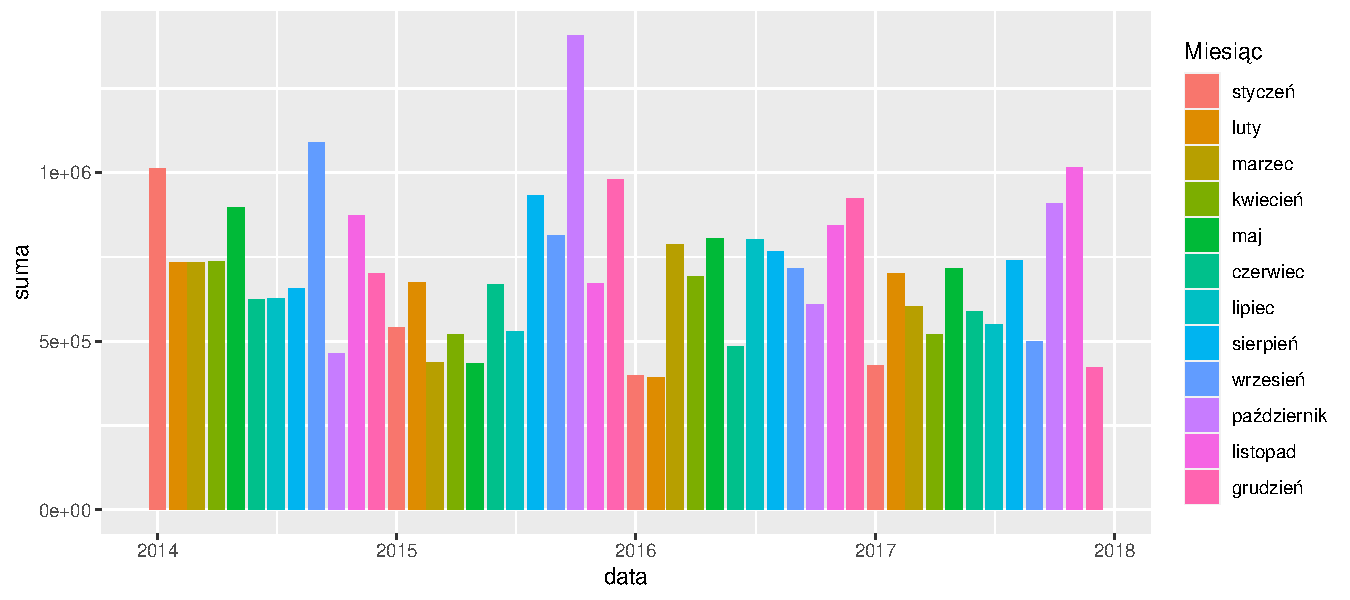
\includegraphics[width=\maxwidth]{figure/fig_zakup_pojazdu-1} 

}

\caption[Miesięczne wydatki na zakup pojazdów]{Miesięczne wydatki na zakup pojazdów}\label{fig:fig_zakup_pojazdu}
\end{figure}

\end{knitrout}

Wykres \ref{fig:fig_zakup_pojazdu} przedstawia miesięczne wydatki na zakup pojazdów. 
Największe wydatki warsztat miał w miesiącu październik 2015. Były one w wysokości 1408.2 tyś. zł. 
Wydatki wielkości 1090.6 tyś. zł były drugimi najwyższymi i były 1.29 razy mniejsze od tych największych. Wystąpiły one w miesiącu wrzesień 2014.
Najmniejsze wydatki warsztat zaobserwował w miesiącu luty 2016 i wyniosły one 392.7 tyś. zł. 
Drugie co do wielkości najniższe wydatki na zakup pojazdów wystąpiły miesiącu styczeń 2016, a wyniosły one 398.5 tyś. zł.
W każdym miesiącu działania warsztatu wydatki na zakup pojazdów wyniosły przynajmnej 400 tyś. zł.

\subsection{Analiza wydatków na zakup części}

Następnie zostało sprawdzone, jak wyglądają miesięczne wydatki na zakup części potrzebnych do napraw pojazdów.

\begin{knitrout}
\definecolor{shadecolor}{rgb}{0.969, 0.969, 0.969}\color{fgcolor}\begin{figure}[H]

{\centering 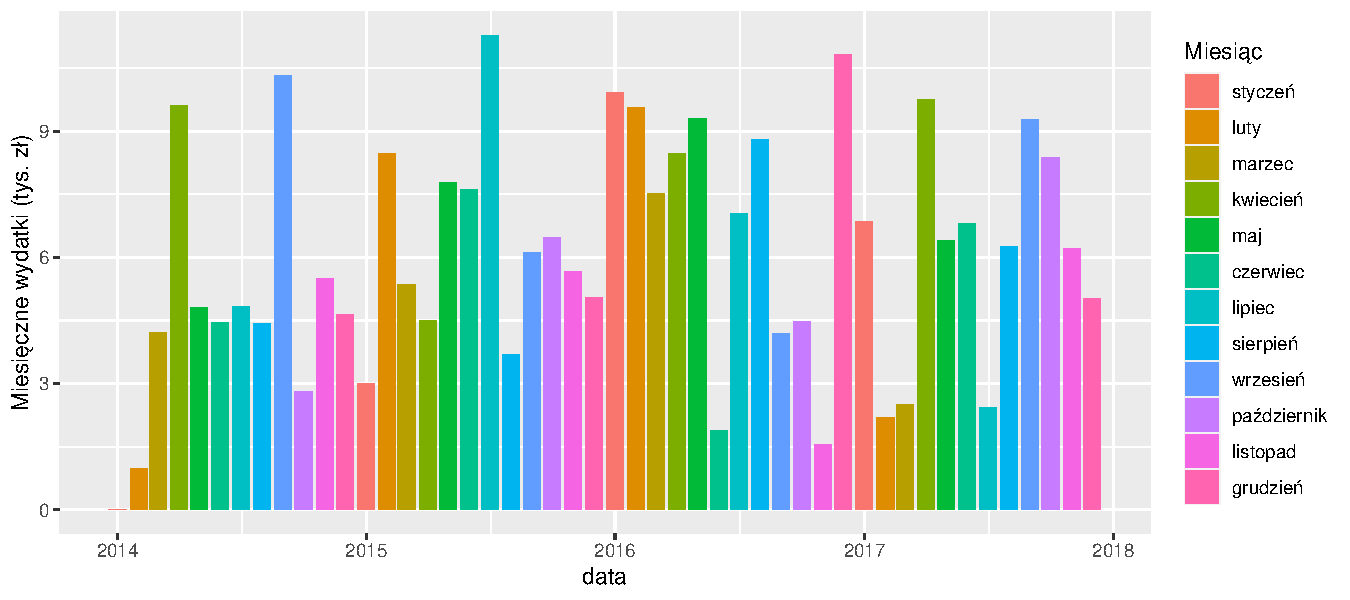
\includegraphics[width=\maxwidth]{figure/fig_zakup_czesci-1} 

}

\caption[Miesięczne wydatki na zakup części]{Miesięczne wydatki na zakup części}\label{fig:fig_zakup_czesci}
\end{figure}

\end{knitrout}

Wykres \ref{fig:fig_zakup_czesci} przedstawia miesięczne wydatki na zakup części do naprawy pojazdów.
Największe wydatki warsztat miał w miesiącu czerwiec 2017 i wyniosły one 16.77 tyś. zł. 
Drugie najwyższye wydatkami były wielkości 16.01 tyś. zł i były 1.05 razy mniejsze od tych największych. Wystąpiły one w miesiącu kwiecień 2014.
Najmniejsze wydatki na części zostały odnotowane w miesiącu styczeń 2014 i wyniosły 0 tyś. zł. 
Drugie najmniejsze wydatki wyniosły 0.97 tyś. zł. Wystąpił on w miesiącu luty 2014.
Ogólnie w każdym miesiącu działania warsztatu wydatki na zakup części wyniosły przynajmnej 0 tyś. zł.

\subsection{Analiza przychodów z usług warsztatu}

Chcielibyśmy sprawdzić, jak wyglądają miesięczne przychody (lub straty) wynikające z prowadzenia warsztatu. Przez przychód za pojedyńczą usługę uważamy różnicę ceny, którą zapłacił klient i kwoty zapłaconej za części. Przeanaliowane zostaną przychody z uwzględnieniem kosztu własnych napraw oraz bez nich.

\begin{knitrout}
\definecolor{shadecolor}{rgb}{0.969, 0.969, 0.969}\color{fgcolor}\begin{figure}[H]

{\centering 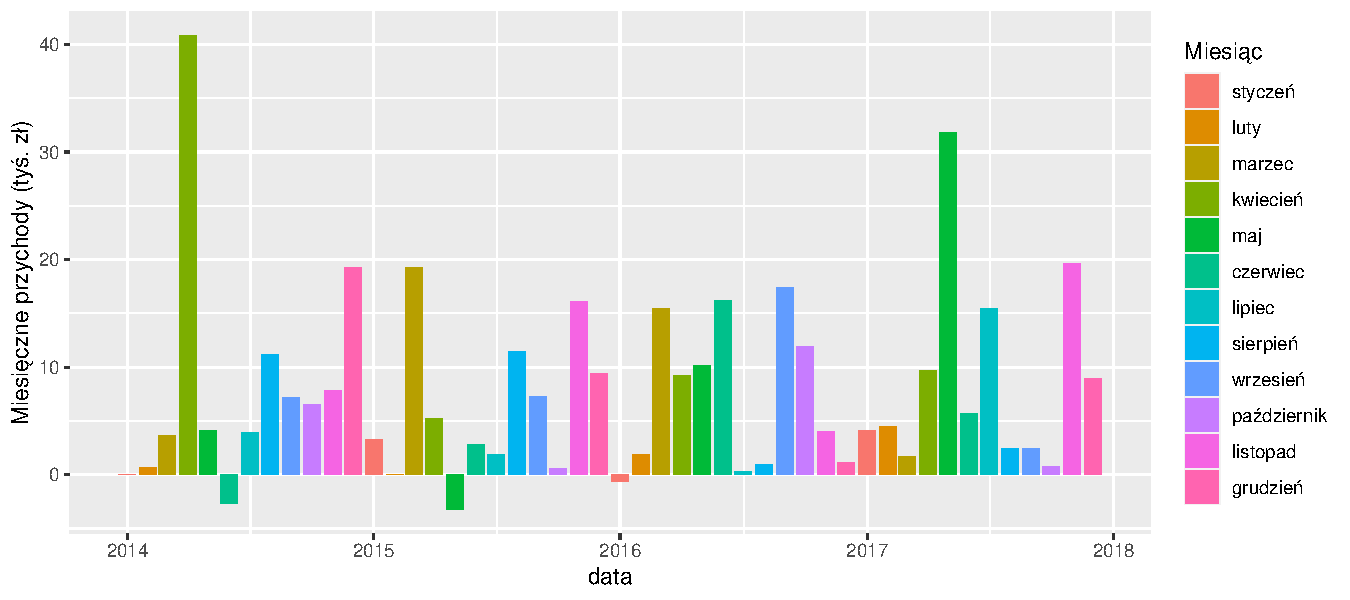
\includegraphics[width=\maxwidth]{figure/fig_uslugi-1} 

}

\caption[Miesięczny przychód wynikający z prowadzenia warsztatu z wliczonymi kosztami napraw własnych]{Miesięczny przychód wynikający z prowadzenia warsztatu z wliczonymi kosztami napraw własnych}\label{fig:fig_uslugi}
\end{figure}

\end{knitrout}

Na wykresie \ref{fig:fig_uslugi} przedstawiony jest miesięczny przychód wynikający z prowadzenia warsztatu. Zostały na nim uwzględnione koszty napraw własnych. 
Największy przychód był zaobserwowany w miesiącu kwiecień 2014 i wyniósł on wtedy 40.86 tyś. zł.
Następny co do wielkości przychód wystąpił w miesiącu maj 2017, wyniósł on 31.85 tyś. zł. Jest on 1.28 razy mniejszy niż najwyższy przychód.
Najmniejszy przychód warsztat odnotował w miesiącu maj 2015, który wyniósł -3.26 tyś. zł. 
Drugi najmniejszy przychód wyniósł -2.65 tyś. zł i wystąpił w miesiącu czerwiec 2014.

\begin{knitrout}
\definecolor{shadecolor}{rgb}{0.969, 0.969, 0.969}\color{fgcolor}\begin{figure}[H]

{\centering 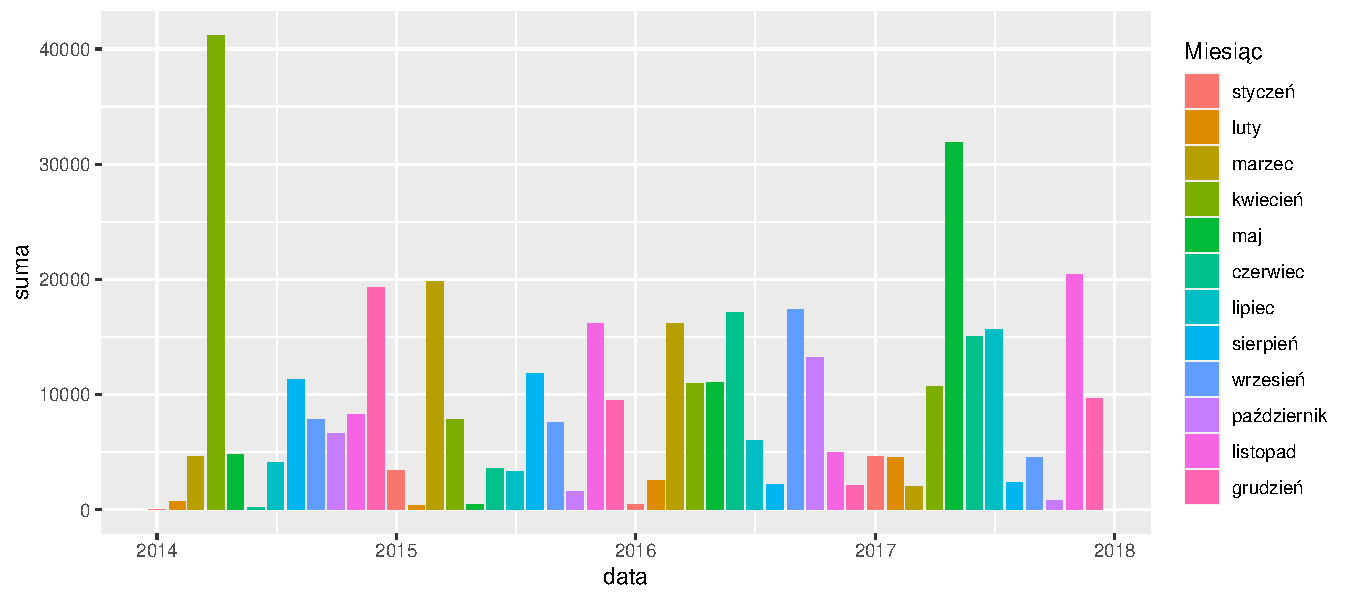
\includegraphics[width=\maxwidth]{figure/fig_uslugi2-1} 

}

\caption[Miesięczny przychód wynikający z prowadzenia warsztatu bez wliczonych kosztów napraw własnych]{Miesięczny przychód wynikający z prowadzenia warsztatu bez wliczonych kosztów napraw własnych}\label{fig:fig_uslugi2}
\end{figure}

\end{knitrout}

Na wykresie \ref{fig:fig_uslugi2} przedstawiony jest miesięczny przychód wynikający z prowadzenia warsztatu, ale tym razem bez uwzględnienia kosztów własnych. 
Największy przychód warsztat zaobserwował w miesiącu kwiecień 2014, który wyniósł 41.2 tyś. zł.
Drugi zaś co do wielkości przychód wsytąpił w miesiącu maj 2017, wyniósł on 31.88 tyś. zł, czyli jest 1.29 razy mniejszy niż ten najwyższy zaobserwowany.
Najmniejszy przychód został odnotowany w miesiącu styczeń 2014 i wyniósł 0 tyś. zł. 
Drugi najmniejszy przychód wyniósł 0.18 tyś. zł. Wystąpił on w miesiącu czerwiec 2014.

\subsection{Koszty wypłat dla pracowników}

Zostanie sprawdzone, jakie miesięczne koszty ponosi warsztat na wypłaty pensji dla pracowników.

%Zakładamy, że płaca w miesiącu to 160*płaca (przy zatrudnieniu/zwolnieniu pracownika patrze ile dni w miesiacu pracownik pracowal i robie ulamek, np. jak zatrudnili go 3 marca to dostaje round(płaca*160*29/31,2)) i podobnie ostatni to by byl round(płaca*160*3/31,2), wypłacamy pieniądze 1 dnia kolejnego miesiąca (np za styczeń wypłacamy 1 lutego)

\begin{knitrout}
\definecolor{shadecolor}{rgb}{0.969, 0.969, 0.969}\color{fgcolor}\begin{figure}[H]

{\centering 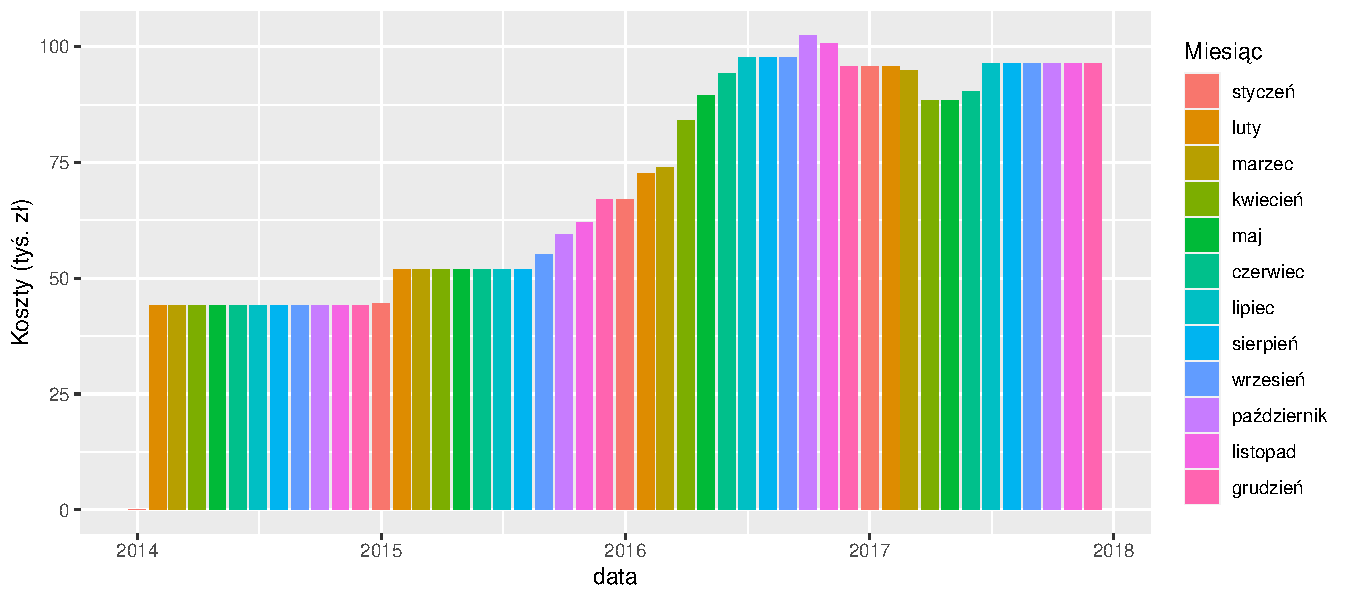
\includegraphics[width=\maxwidth]{figure/fig_pracownicy-1} 

}

\caption[Miesięczne koszty wynikające z wypłacania pensji pracownikom]{Miesięczne koszty wynikające z wypłacania pensji pracownikom}\label{fig:fig_pracownicy}
\end{figure}

\end{knitrout}

Wykres \ref{fig:fig_pracownicy} przedstawia miesięczne koszty wypłat pensji pracowników. Największy koszt warsztat odnotował w miesiącu październik 2016 i wyniósł on 102.49 tyś. zł. 
Natomiast najmniejsze koszty wystąpiły w miesiącu styczeń 2014. Wyniosły one 0 zł. Wynika to z tego, że jest to pierwszy miesiąc działania warsztatu, a pensje wypłacamy pracownikom pierwszego dnia następnego miesiąca.. Poza tym miesiącem najmniej wypłacono pracownikom w miesiącu luty 2014. Była to kwota 44.03 tyś. zł

\subsection{Wpływy ze sprzedaży pojazdów}

Następnie zostaną sprawdzone miesięczne wpływy finansowe ze sprzedaży pojazdów, które zostały zakupione i w razie potrzeby naprawione przez warsztat. Pojazdy są sprzedawane na dwa sposoby: klient może zapłacić całą kwotę na raz lub spłacać w ratach.

\begin{knitrout}
\definecolor{shadecolor}{rgb}{0.969, 0.969, 0.969}\color{fgcolor}\begin{figure}[H]

{\centering 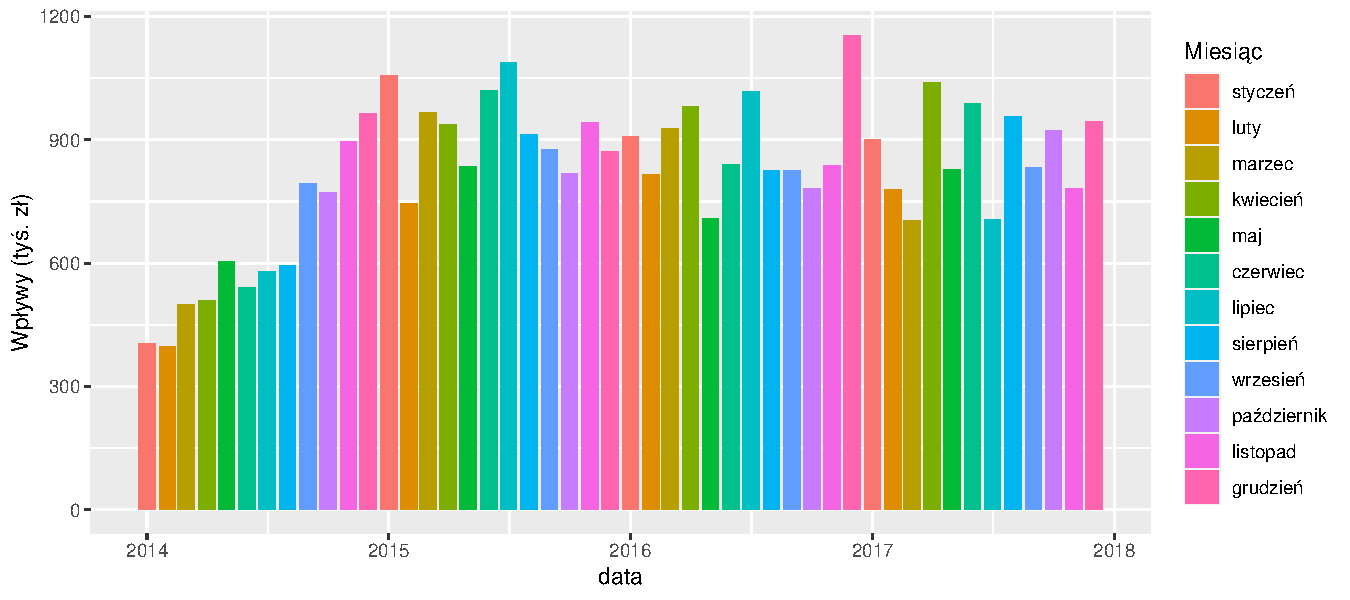
\includegraphics[width=\maxwidth]{figure/fig_samochody_wplywy-1} 

}

\caption[Miesięczne wpływy finansowe ze sprzedaży pojazdów]{Miesięczne wpływy finansowe ze sprzedaży pojazdów}\label{fig:fig_samochody_wplywy}
\end{figure}

\end{knitrout}

Na wykresie \ref{fig:fig_samochody_wplywy} przedstawione są wpływy finansowe ze sprzedaży pojazdów. 
Największe miesięczne wpływy warsztatu ze sprzedaży pojazdów wynosiły 1.24 mln. zł. Wystąpiły one w miesiącu grudzień 2015. 
Drugie co do wielkości wpływy (w wysokości 1.17 mln. zł) zostały odnotowane w miesiącu kwiecień 2017. Są one 1.06 razy mniejsze niż te największe zaobserwowane.
Najmniejsze miesięczne wpływy wyniosły 0.32 mln. zł, a wystąpiły one w miesiącu marzec 2014.
Kolejnymi najmniejszymi są wpływy z miesiącu styczeń 2014. Są one wysokości 0.36 mln. zł.


\subsection{Bilans miesięczny}

Teraz zostanie sprawdzoby miesięczny bilans warsztatu. Zostaną sprawdzone miesięczne przychody warsztaty przez cały okres jego działania oraz comiesięczny stan środków finansowych firmy, gdyby warsztat zaczynał bez posiadania żadnych średków pienięznych.

\begin{knitrout}
\definecolor{shadecolor}{rgb}{0.969, 0.969, 0.969}\color{fgcolor}\begin{figure}[H]

{\centering 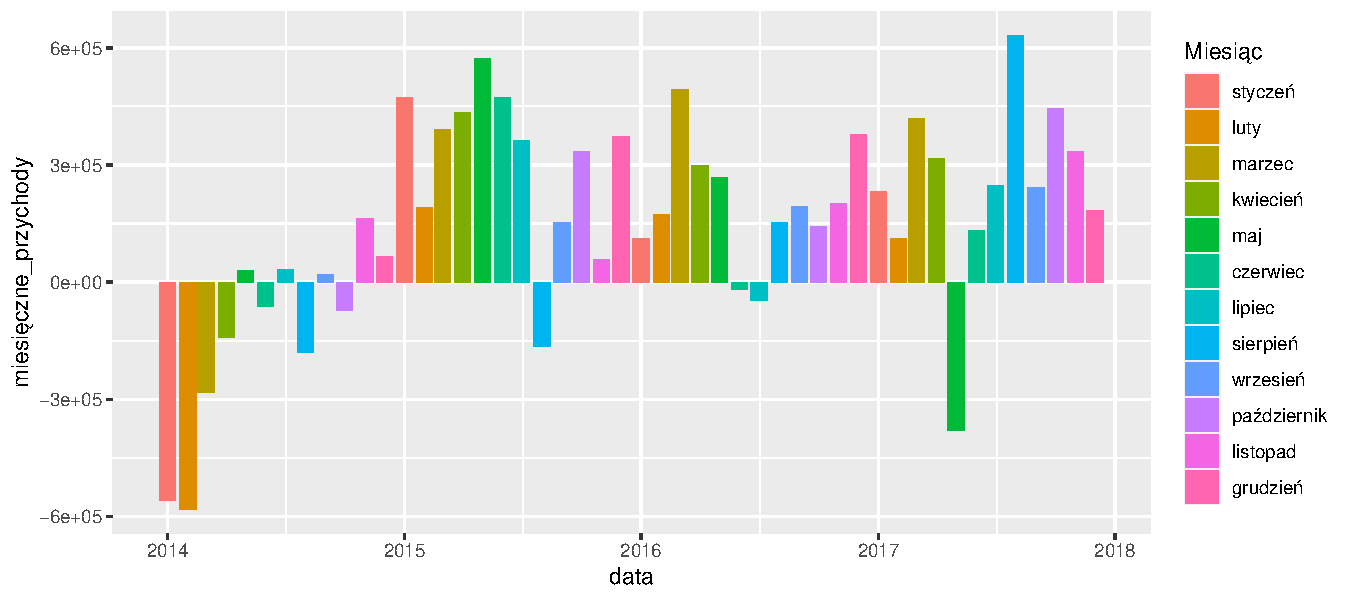
\includegraphics[width=\maxwidth]{figure/fig_bilans-1} 

}

\caption[Miesięczne przychody warsztatu]{Miesięczne przychody warsztatu}\label{fig:fig_bilans}
\end{figure}

\end{knitrout}

%złączenie: na miesiąc = naprawy(te z minusami, bo mają razem części) + sprzedaż pojazdu -zakup pojazdu - wypłaty (czy ja coś pominęłam?)

Wykres \ref{fig:fig_bilans} przedstawia miesięczne przychody firmy od początku jej działalności. 
Najwięcej warsztat zarobił (702.95 tyś. zł) w miesiącu styczeń 2016.
Natomiast najmniej w miesiącu styczeń 2014. Zyski wyniosły wtedy -650.09 tyś. zł. Przez pierwsze 3 miesięcy pracy warsztat nie przynosił żadnych zysków.

\begin{knitrout}
\definecolor{shadecolor}{rgb}{0.969, 0.969, 0.969}\color{fgcolor}\begin{figure}[H]

{\centering 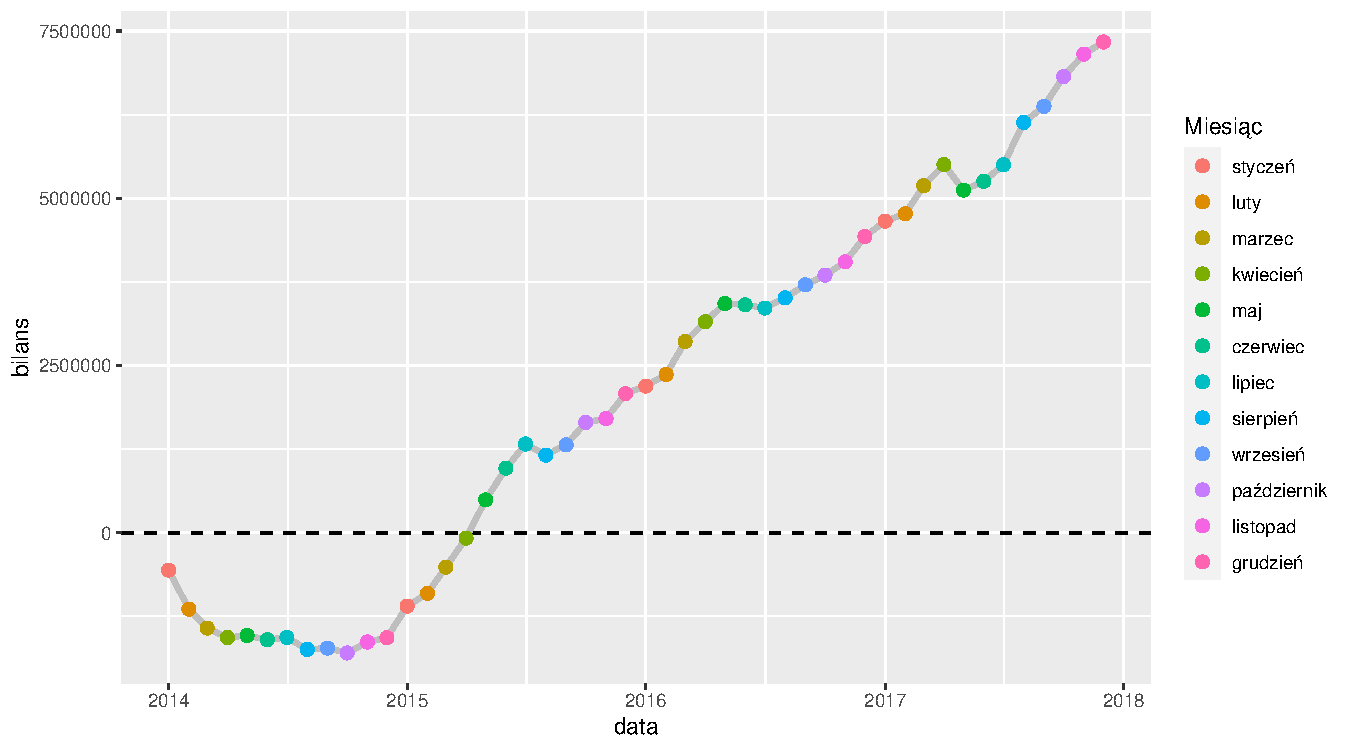
\includegraphics[width=\maxwidth]{figure/fig_bilans_suma-1} 

}

\caption[Miesięczny stan finansowy warsztatu, gdyby zaczynał działalność bez żadnych środków pieniężnych]{Miesięczny stan finansowy warsztatu, gdyby zaczynał działalność bez żadnych środków pieniężnych}\label{fig:fig_bilans_suma}
\end{figure}

\end{knitrout}

Wykres \ref{fig:fig_bilans_suma} przedstawia miesięczny stan finansowy warsztatu, gdyby zaczynał działalność bez środków pieniężnych. W pierwszym miesiącu działalności stan finansowy wyniósł -0.65 mln. zł, natomiast aktualnie wynosi on 6.91 mln. zł. Przez pierwsze 14 miesięcy pracy warsztatu jego stan finansowy był ujemny.
Największą ilością pieniędzy warsztat operował w miesiącu grudzień 2017, było to 6.91 mln. zł.
Natomiast najmniejszą w miesiącu wrzesień 2014, a było to -1.82 mln. zł.

\section{Podsumowanie}





\end{document}
